\begin{figure}[h]
 \begin{minipage}[b]{0.48\linewidth}
  \centering
  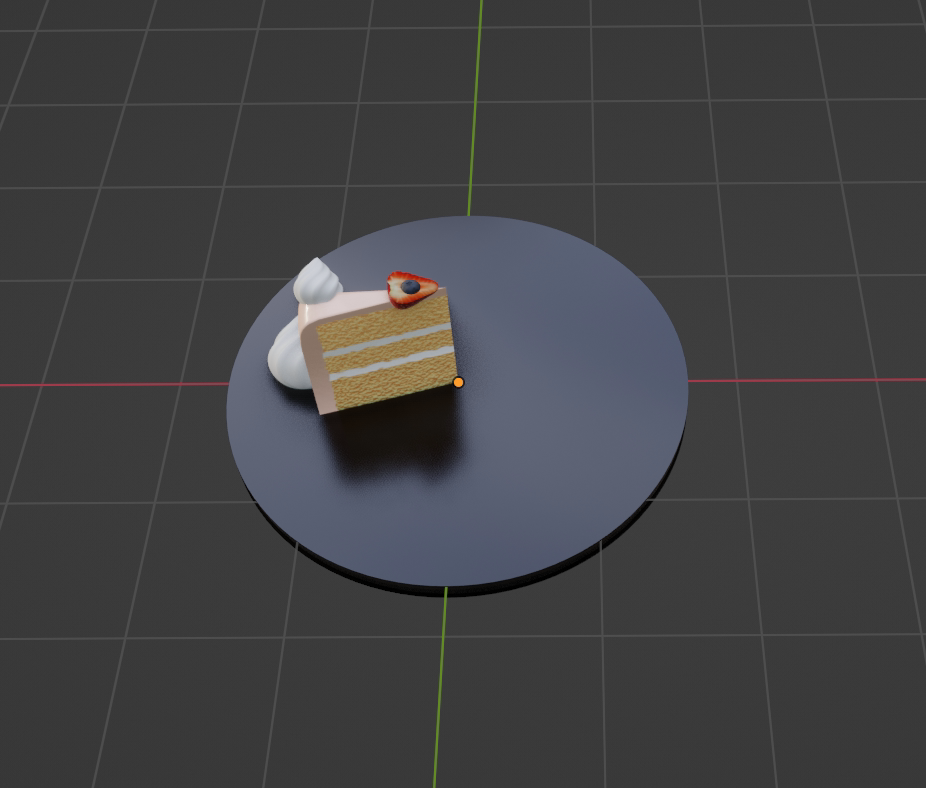
\includegraphics[scale=0.25]{./imgs/cakeParamMean/cutMin.png}
        \subcaption{Cake cut 最小(0.0)}
 \end{minipage}
 \begin{minipage}[b]{0.48\linewidth}
  \centering
  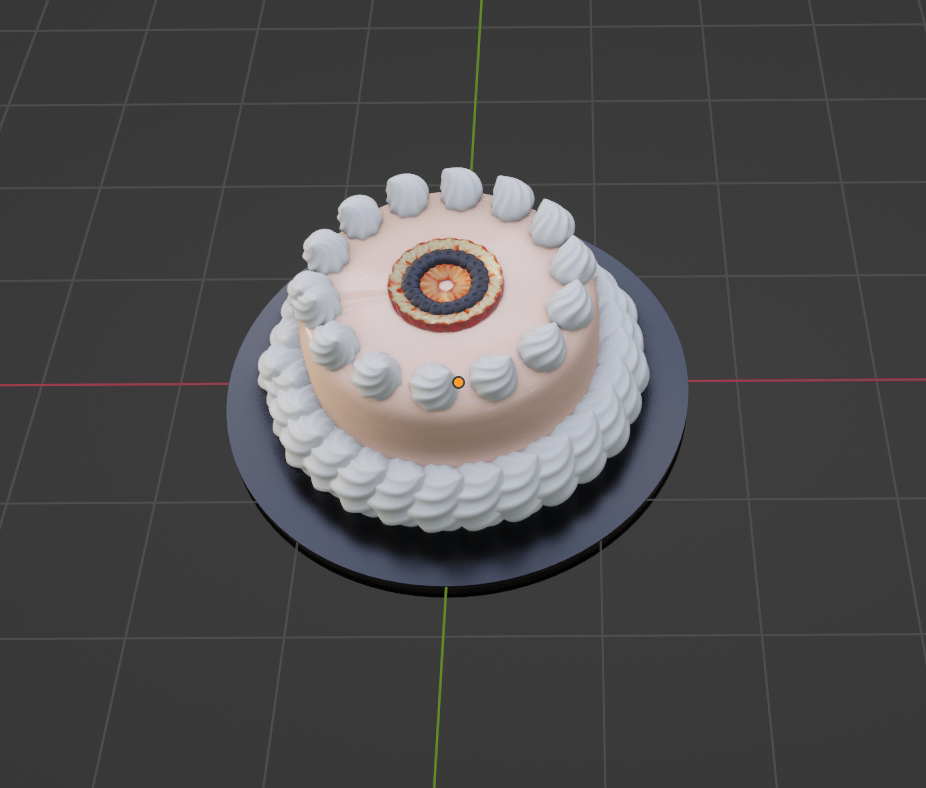
\includegraphics[scale=0.25]{./imgs/cakeParamMean/cutMax.png}
        \subcaption{Cake cut 最大(1.0)}
 \end{minipage}\\
 \begin{minipage}[b]{0.48\linewidth}
  \centering
  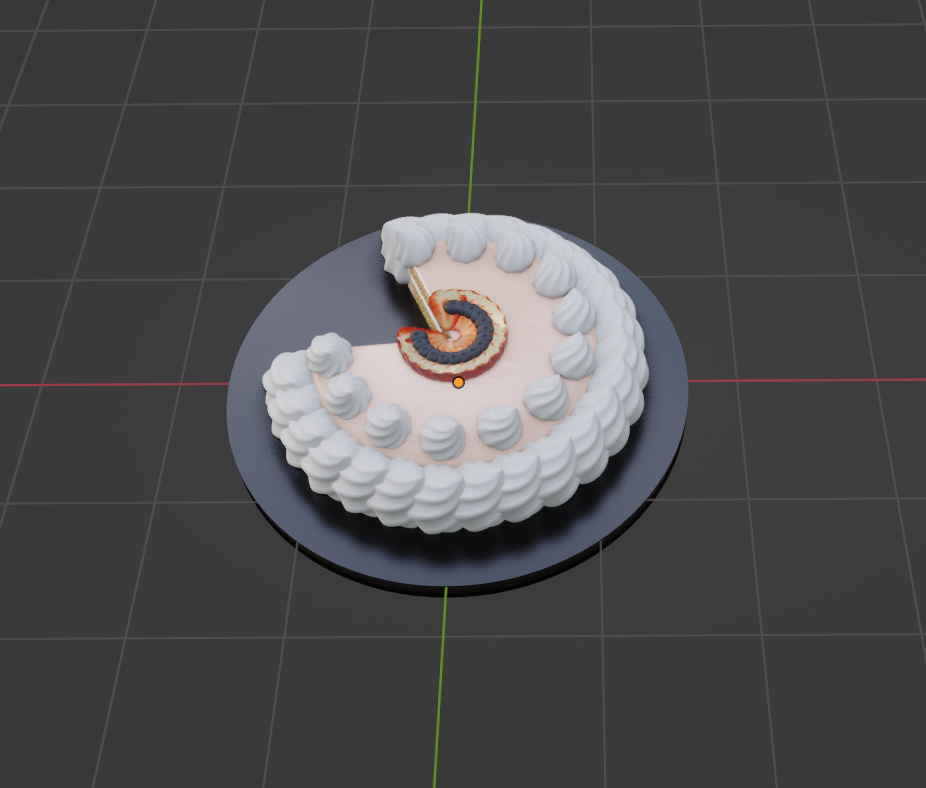
\includegraphics[scale=0.25]{./imgs/cakeParamMean/heightMin.png}
        \subcaption{Cake height 最小(0.5)}
 \end{minipage}
 \begin{minipage}[b]{0.48\linewidth}
  \centering
  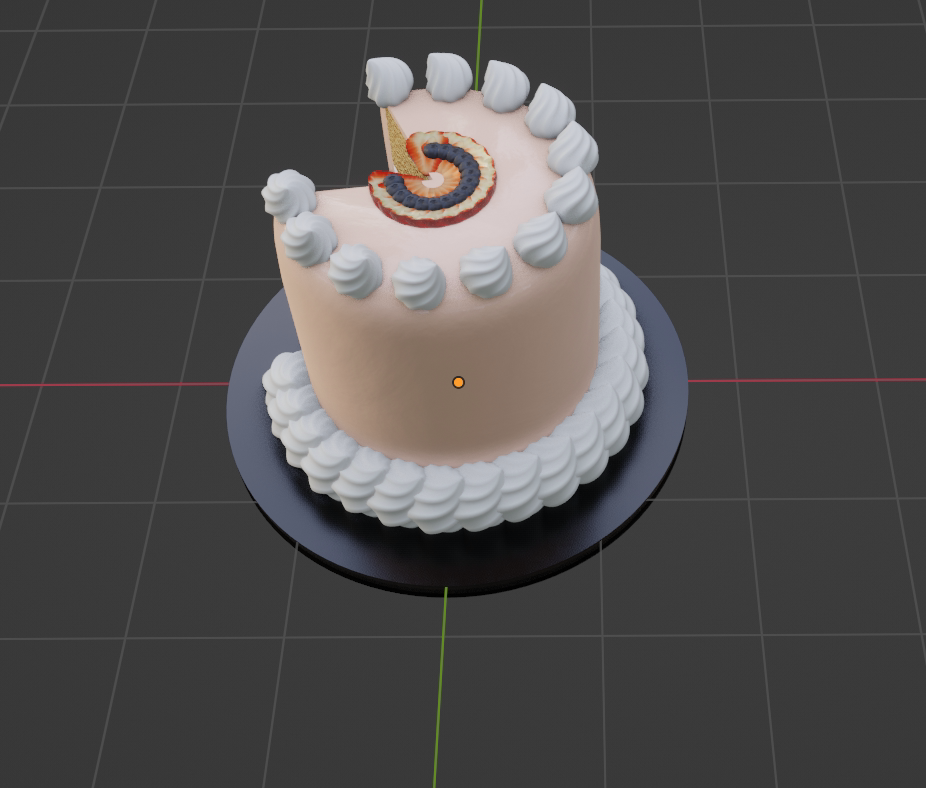
\includegraphics[scale=0.25]{./imgs/cakeParamMean/heightMax.png}
        \subcaption{Cake height 最大(2.0)}
 \end{minipage}
 \caption{Cake モデルにおけるパラメータ範囲(1)}\label{fig:cakeParamMean_1}
\end{figure}

\begin{figure}[h]
 \begin{minipage}[b]{0.48\linewidth}
  \centering
  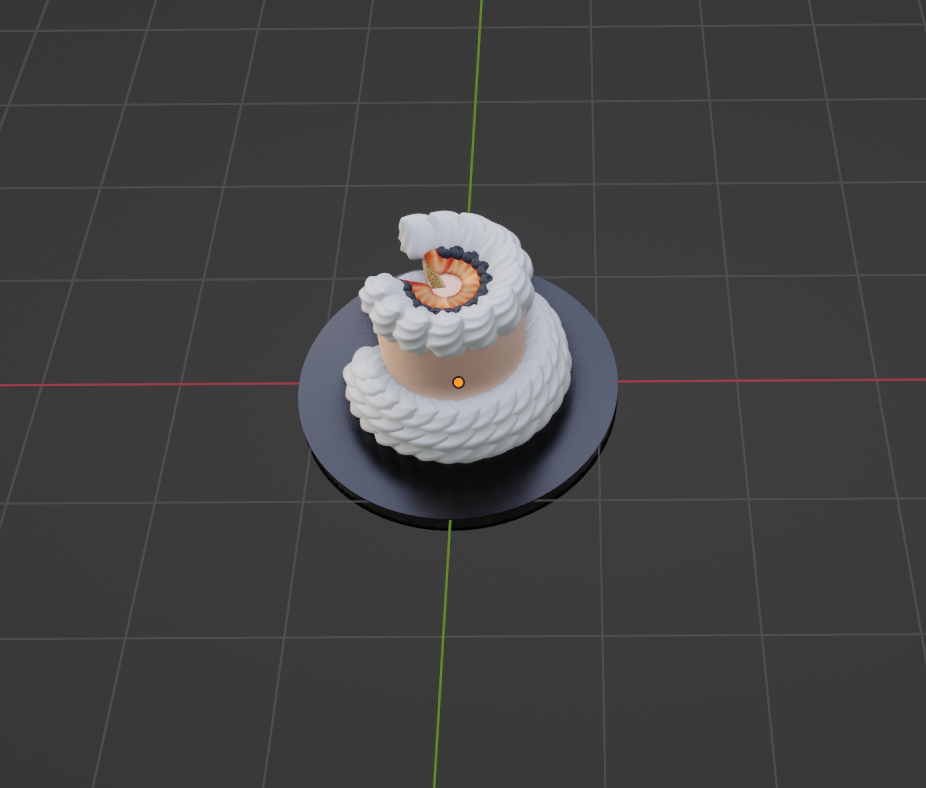
\includegraphics[scale=0.25]{./imgs/cakeParamMean/radiusMin.png}
        \subcaption{Cake radius 最小(0.0)}
 \end{minipage}
 \begin{minipage}[b]{0.48\linewidth}
  \centering
  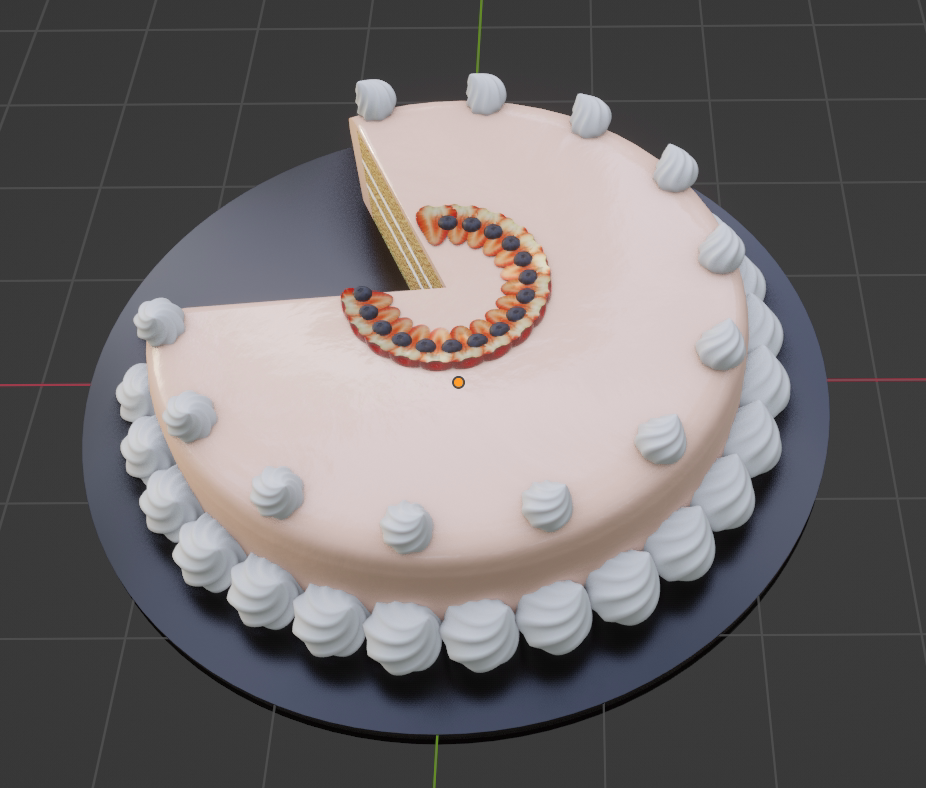
\includegraphics[scale=0.25]{./imgs/cakeParamMean/radiusMax.png}
        \subcaption{Cake radius 最大(1.0)}
 \end{minipage}\\
  \begin{minipage}[b]{0.48\linewidth}
  \centering
  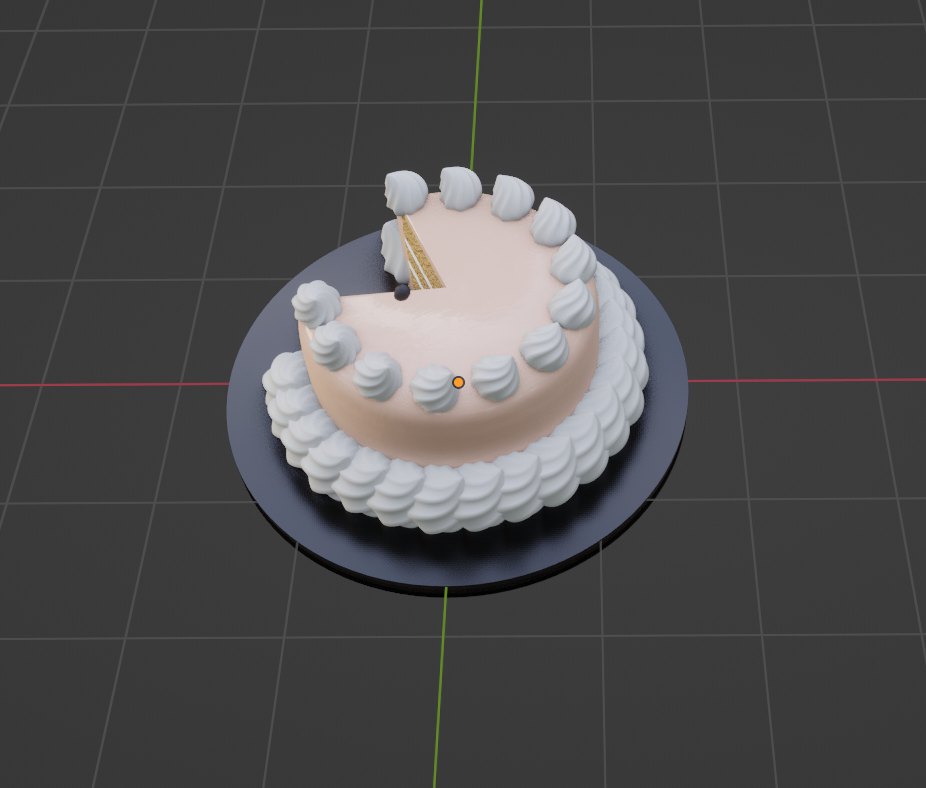
\includegraphics[scale=0.25]{./imgs/cakeParamMean/toppingQuanMin.png}
        \subcaption{Topping quantity 最小(0.0)}
 \end{minipage}
 \begin{minipage}[b]{0.48\linewidth}
  \centering
  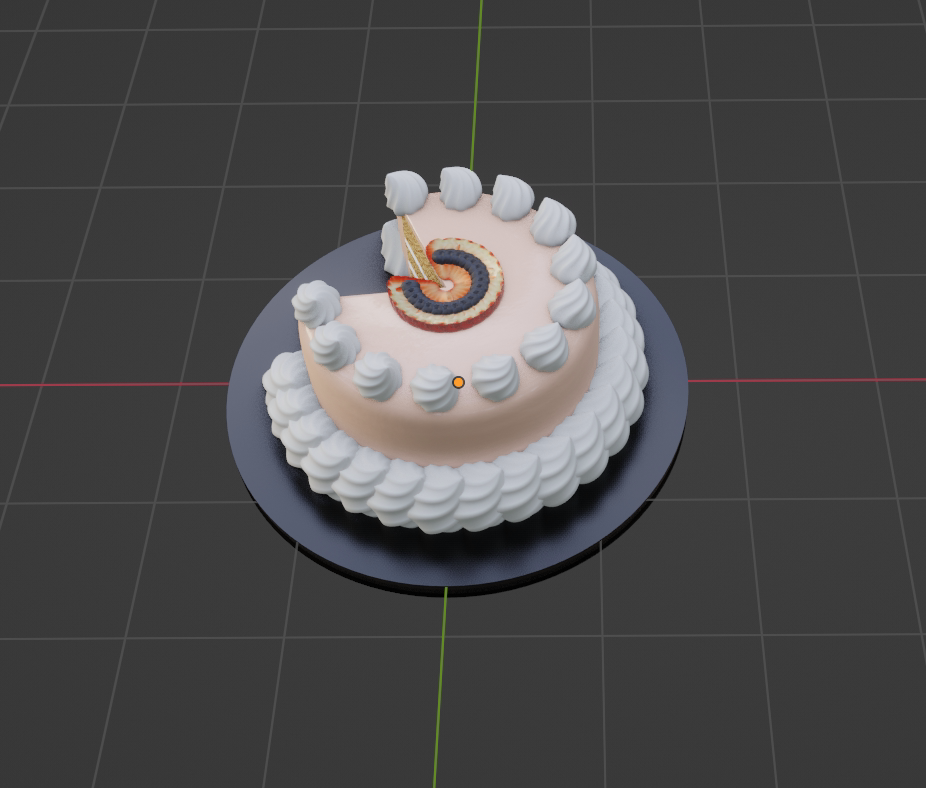
\includegraphics[scale=0.25]{./imgs/cakeParamMean/toppingQuanMax.png}
        \subcaption{Topping quantity 最大(50.0)}
 \end{minipage}\\
 \begin{minipage}[b]{0.48\linewidth}
  \centering
  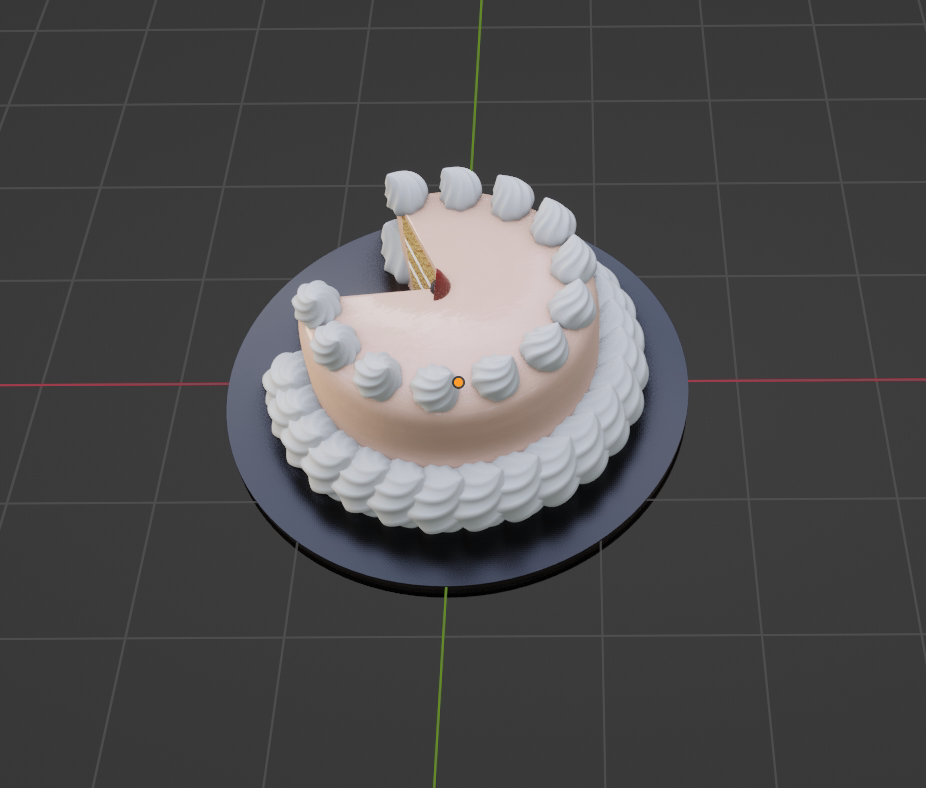
\includegraphics[scale=0.25]{./imgs/cakeParamMean/toppingPosMin.png}
        \subcaption{Topping position 最小(0.0)}
 \end{minipage}
 \begin{minipage}[b]{0.48\linewidth}
  \centering
  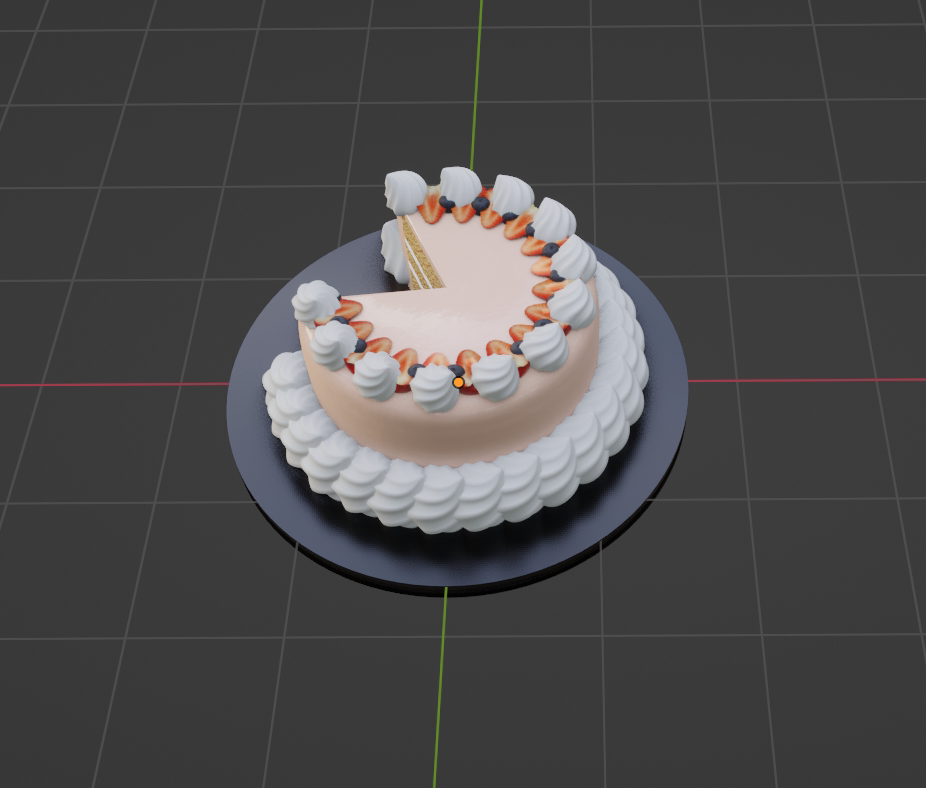
\includegraphics[scale=0.25]{./imgs/cakeParamMean/toppingPosMax.png}
        \subcaption{Topping position 最大(1.0)}
 \end{minipage}
 \caption{Cake モデルにおけるパラメータ範囲(2)}\label{fig:cakeParamMean_2}
\end{figure}

\begin{figure}[h]
 \begin{minipage}[b]{0.48\linewidth}
  \centering
  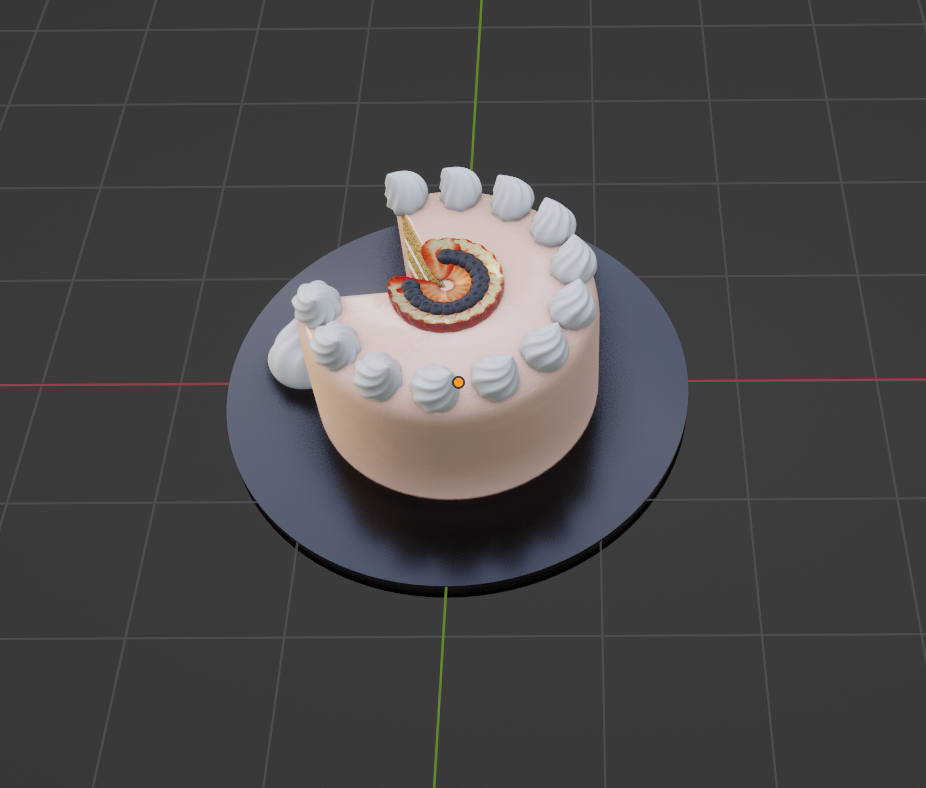
\includegraphics[scale=0.25]{./imgs/cakeParamMean/botQuanMin.png}
        \subcaption{CreamBot quantity 最小(0.0)}
 \end{minipage}
 \begin{minipage}[b]{0.48\linewidth}
  \centering
  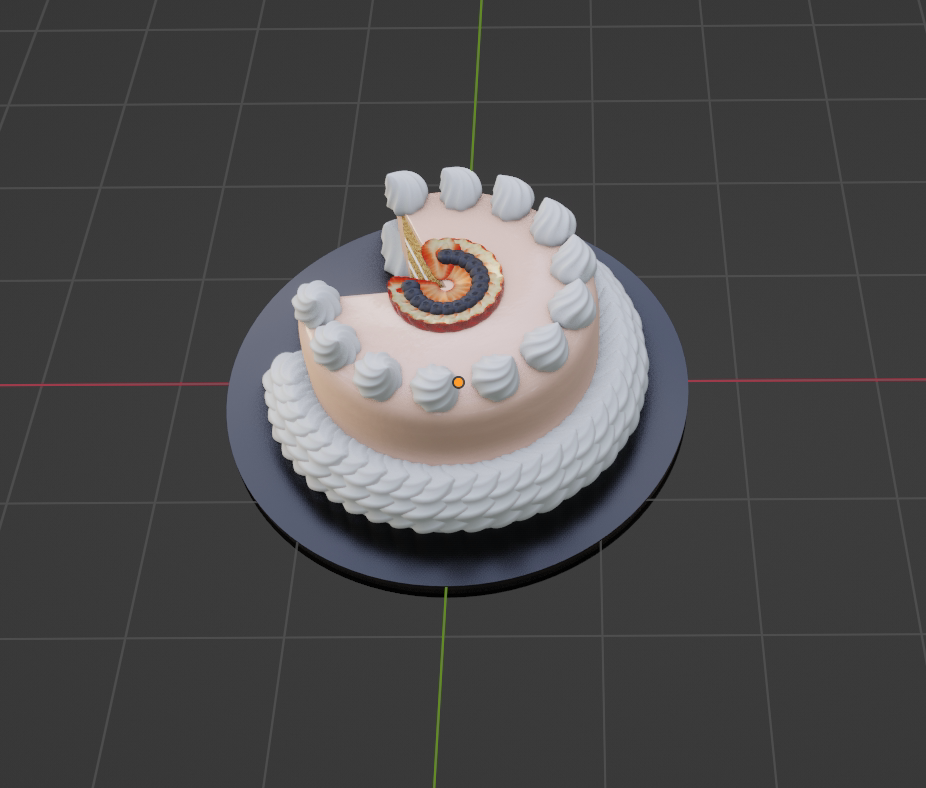
\includegraphics[scale=0.25]{./imgs/cakeParamMean/botQuanMax.png}
        \subcaption{CreamBot quantity 最大(50.0)}
 \end{minipage}\\
  \begin{minipage}[b]{0.48\linewidth}
  \centering
  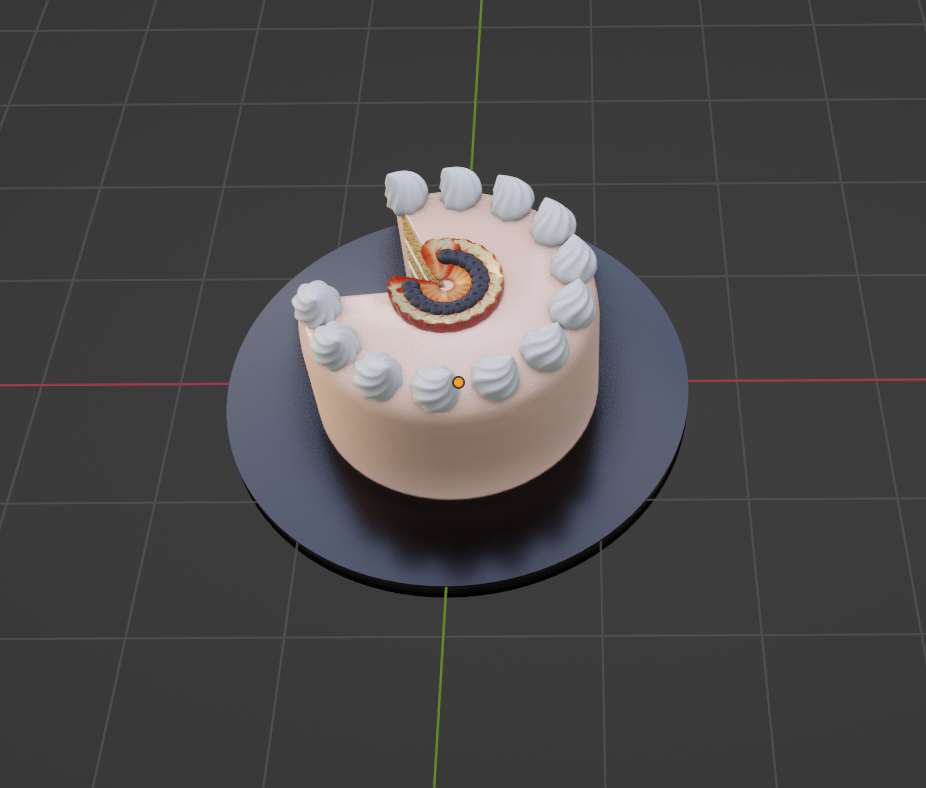
\includegraphics[scale=0.25]{./imgs/cakeParamMean/botSizeMin.png}
        \subcaption{CreamBot size 最小(0.0)}
 \end{minipage}
 \begin{minipage}[b]{0.48\linewidth}
  \centering
  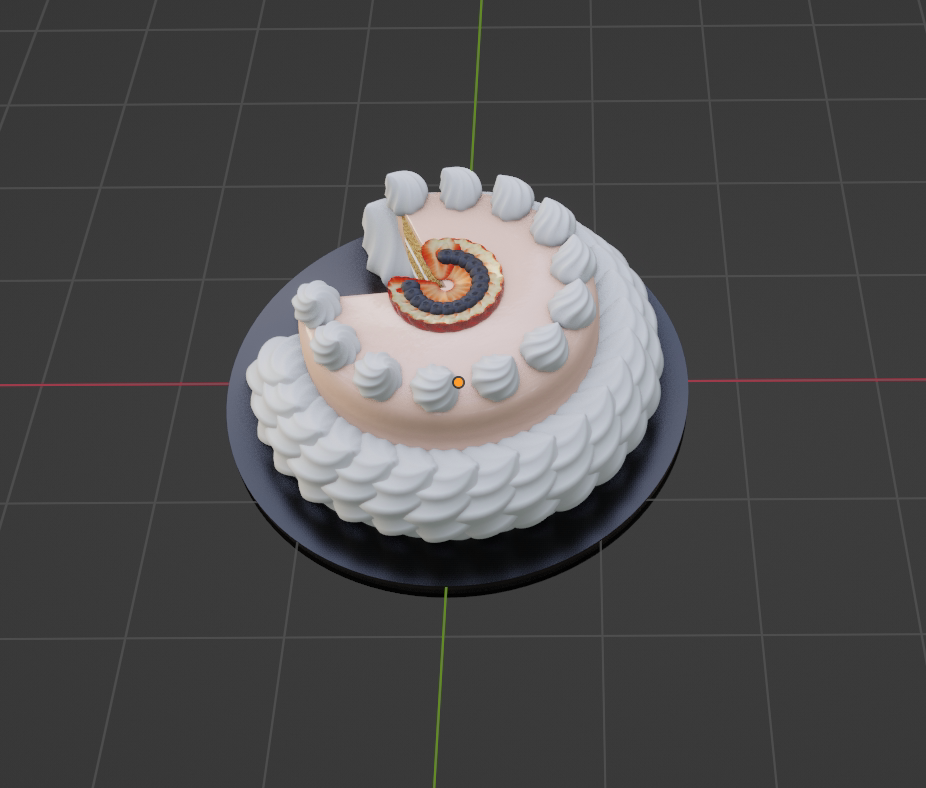
\includegraphics[scale=0.25]{./imgs/cakeParamMean/botSizeMax.png}
        \subcaption{CreamBot size 最大(2.0)}
 \end{minipage}\\
 \begin{minipage}[b]{0.48\linewidth}
  \centering
  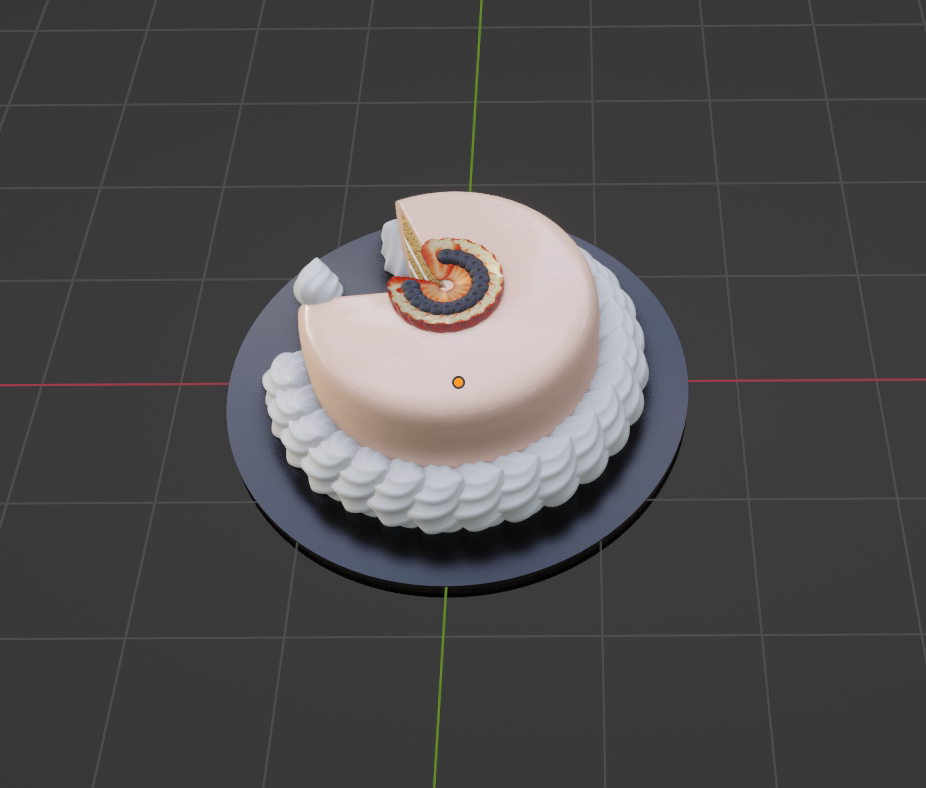
\includegraphics[scale=0.25]{./imgs/cakeParamMean/topQuanMin.png}
        \subcaption{CreamTop quantity 最小(0.0)}
 \end{minipage}
 \begin{minipage}[b]{0.48\linewidth}
  \centering
  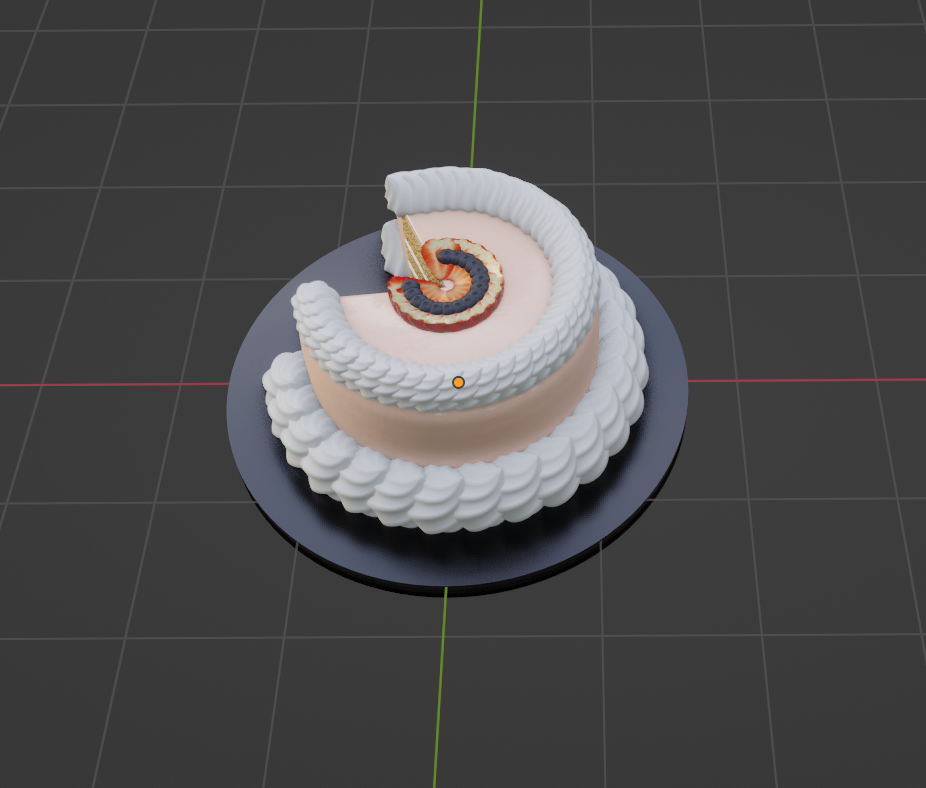
\includegraphics[scale=0.25]{./imgs/cakeParamMean/topQuanMax.png}
        \subcaption{CreamTop quantity 最大(50.0)}
 \end{minipage}
 \caption{Cake モデルにおけるパラメータ範囲(3)}\label{fig:cakeParamMean_3}
\end{figure}


\begin{figure}[h]
 \begin{minipage}[b]{0.48\linewidth}
  \centering
  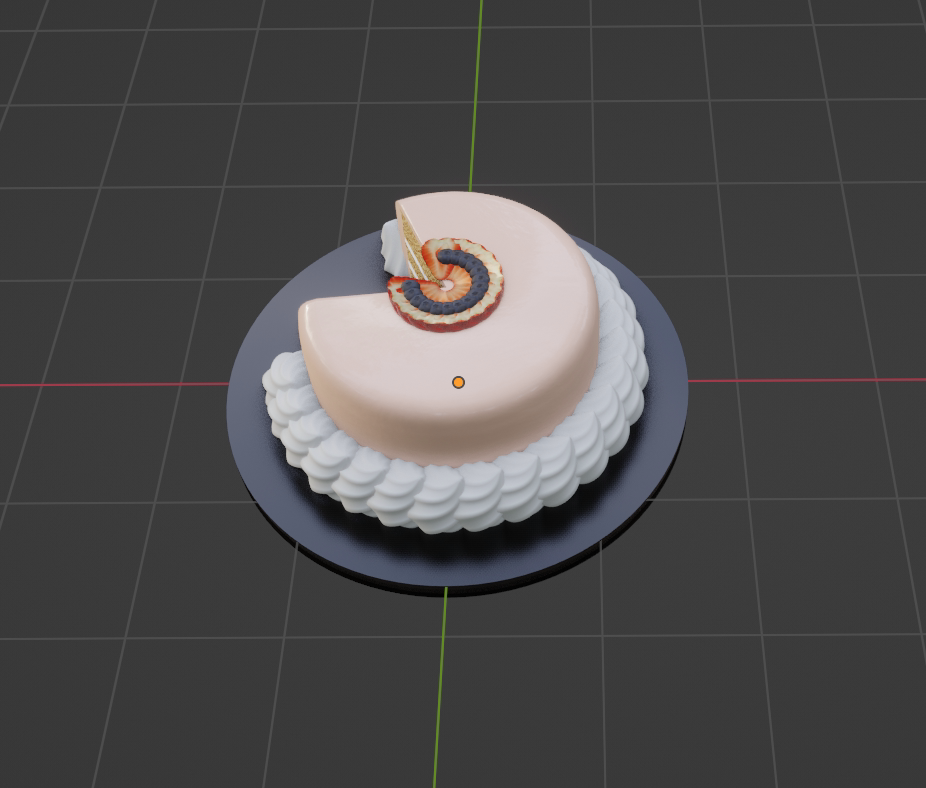
\includegraphics[scale=0.25]{./imgs/cakeParamMean/topSizeMin.png}
        \subcaption{CreamTop size 最小(0.0)}
 \end{minipage}
 \begin{minipage}[b]{0.48\linewidth}
  \centering
  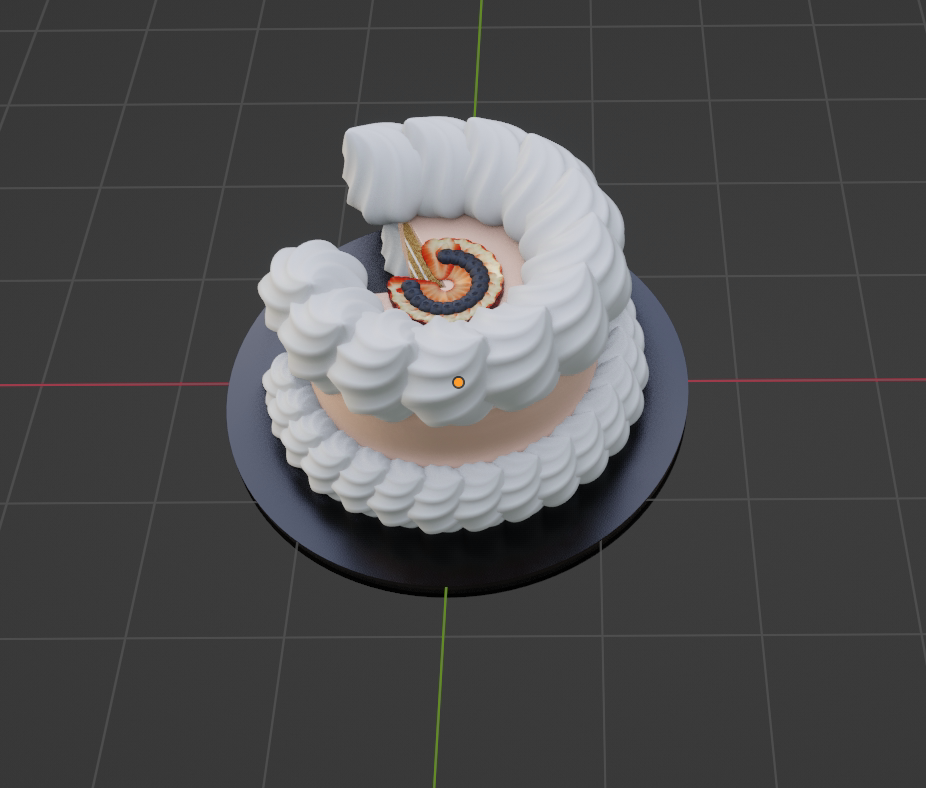
\includegraphics[scale=0.25]{./imgs/cakeParamMean/topSizeMax.png}
        \subcaption{CreamTop size 最大(2.0)}
 \end{minipage}\\
 \begin{minipage}[b]{0.48\linewidth}
  \centering
  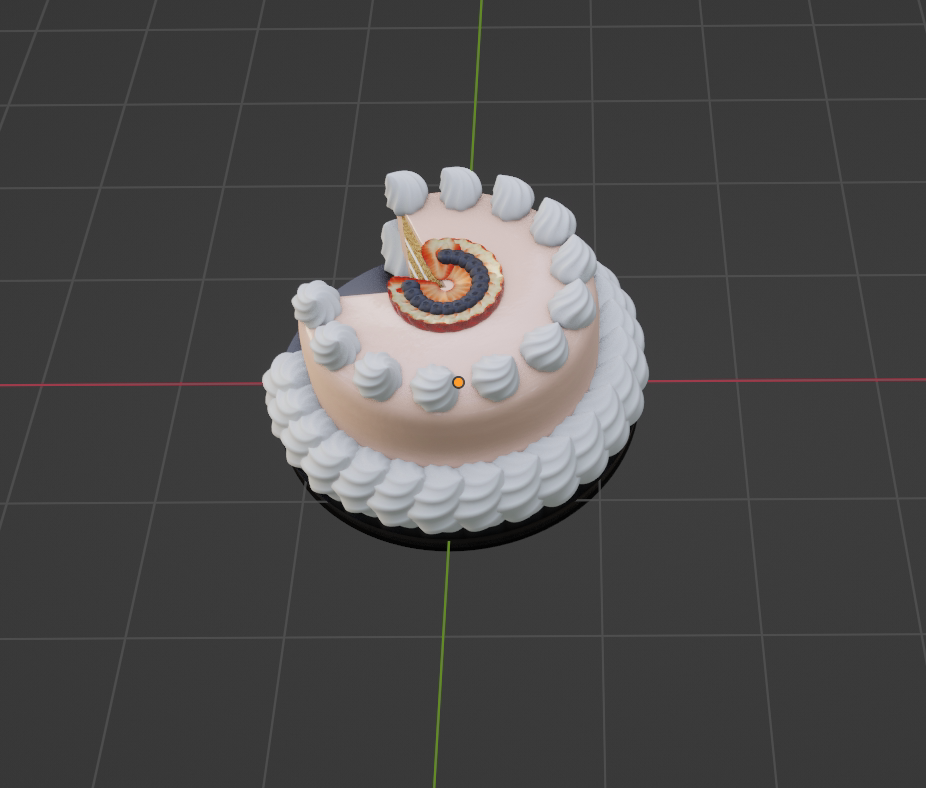
\includegraphics[scale=0.25]{./imgs/cakeParamMean/plateSizeMin.png}
        \subcaption{Plate size 最小(0.3)}
 \end{minipage}
 \begin{minipage}[b]{0.48\linewidth}
  \centering
  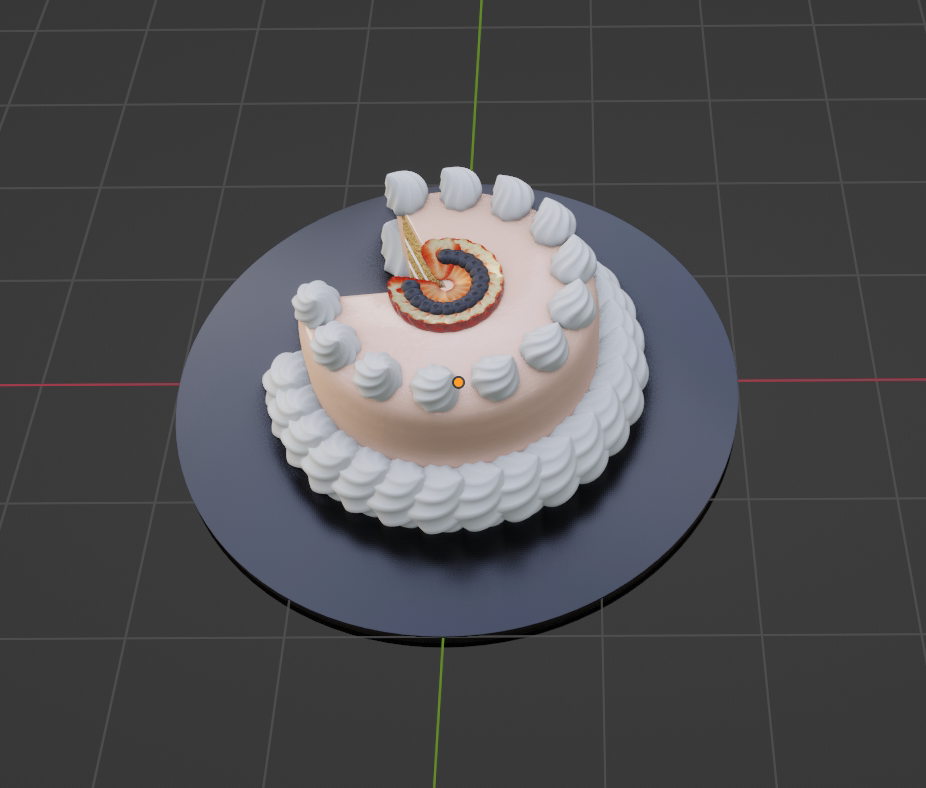
\includegraphics[scale=0.25]{./imgs/cakeParamMean/plateSizeMax.png}
        \subcaption{Plate size 最大(1.0)}
 \end{minipage}\\
 \begin{minipage}[b]{0.48\linewidth}
  \centering
  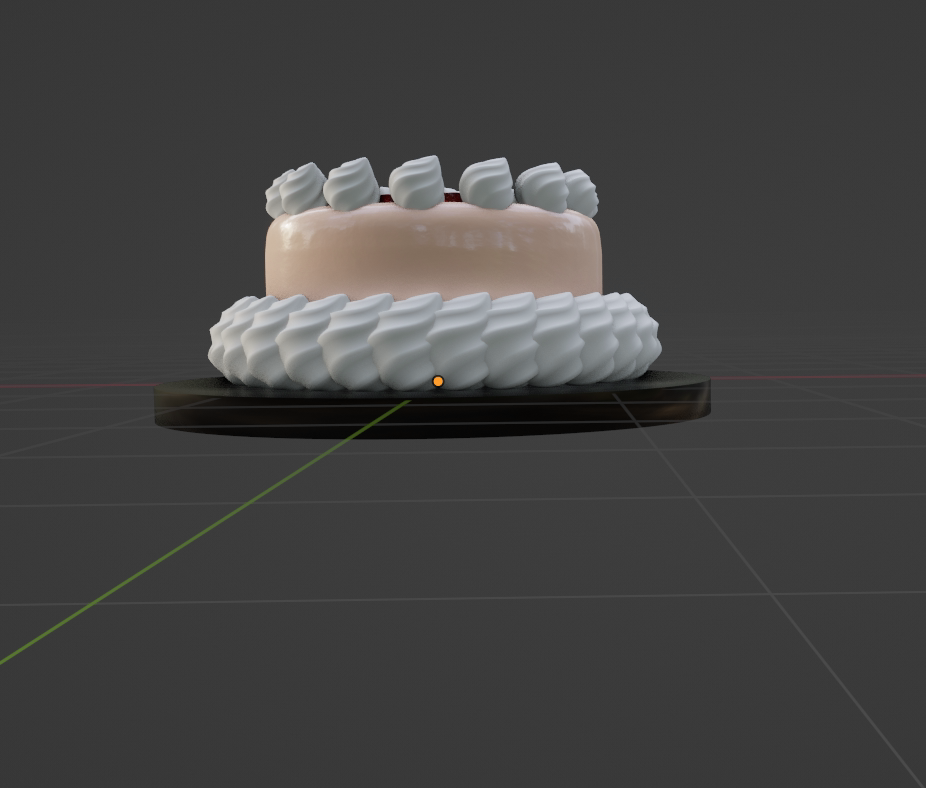
\includegraphics[scale=0.25]{./imgs/cakeParamMean/tickMin.png}
        \subcaption{Plate thickness 最小(-0.2)}
 \end{minipage}
 \begin{minipage}[b]{0.48\linewidth}
  \centering
  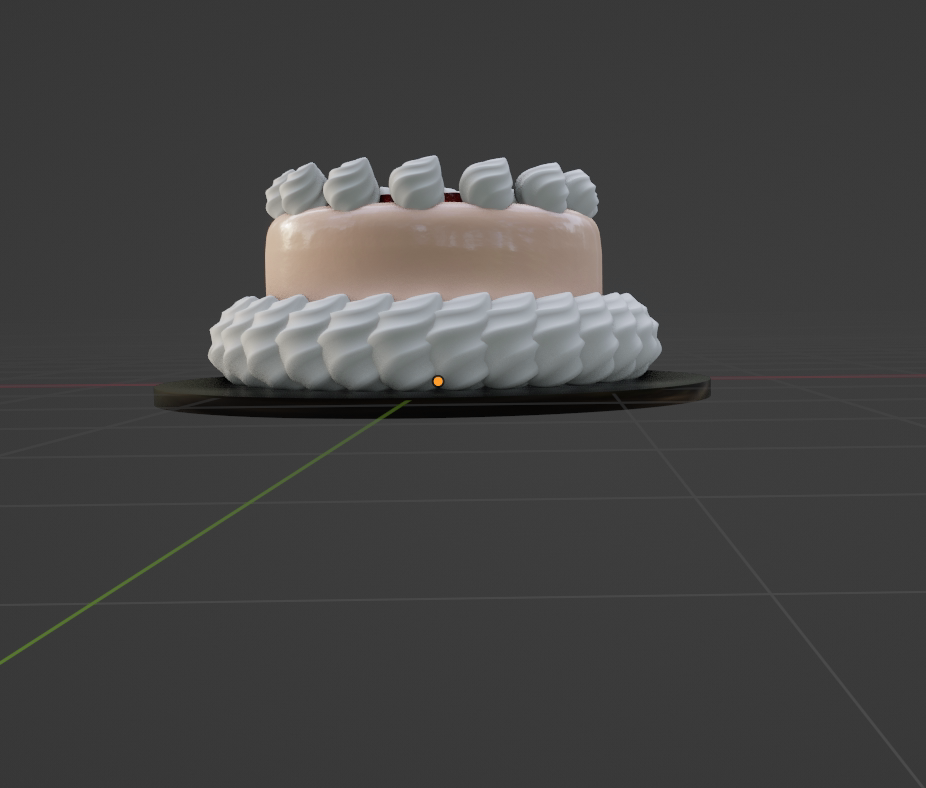
\includegraphics[scale=0.25]{./imgs/cakeParamMean/tickMax.png}
        \subcaption{Plate thickness 最大(-0.1)}
 \end{minipage}
 \caption{Cake モデルにおけるパラメータ範囲(4)}\label{fig:cakeParamMean_4}
\end{figure}